%
Als ersten Schritt der digitalen Signalverarbeitung wollen wir uns den \"Ubergang von einem analogen Signal zu einem digitalen n\"aher ansehen.
Intuitiv k\"onnen wir diesen Vorgang in vielen Anwendungen beobachten.
Wir nehmen im Tonstudio mit einem Mikrophon Ton auf und eine Soundkarte wandelt das analoge Signal in einen WAV-Datenstrom um.
In einer Fotokamera, trifft ein Feld von Lichtstrahlen ein und wird von einem CMOS-Sensor \q{direkt} abgetastet und in Helligkeitswerte pro Farbkanal umgewandelt.
Eine Antenne wandelt ein anliegendes elektro-magnetisches Feld in eine Spannung um, welche nachtr\"aglich von einem \gls{adc} abgetastet und quantisiert wird.

Mathematisch modellieren wir analoge Signale $s_a : D \rightarrow B$ meist mit $D$ und $B$, die auf die reellen Zahlen $\R$ zur\"uckgreifen.
Die Wandlung von analog zu digital transformiert dieses Signal in eine Funktion $s: \Z \rightarrow Q$ um, wobei auch $\Abs{Q} < \infty$ gilt.
Das hei\ss{}t, dass das Signal nach AD-Wandlung nur noch endliche Werte annehmen kann und, dass es nur noch aus eine \emph{Folge} von Werten aus der Menge $Q$ besteht. 
Es wurde also zeit- und wertdiskretisiert.
Wir werden uns zun"achst nur mit der Diskretisierung in Zeit befassen, weil es einfach einfacher ist.
Das hei"st, dass wir uns vorstellen, dass das diskretisierte Signal nur an einer diskreten Menge an Punkten noch Informationen "uber das abgetastete Signal beinhaltet.
Weiterhin sind wir nicht an der physikalischen Umsetzung von \glspl{adc} interessiert, sondern h"ochstens an deren systemtheoretischer Modellierung.

Die zentralen Fragen sind nun:
\begin{itemize}
    \item Wie muss der Vorgang der Abtastung gestaltet sein, dass keine Information verloren geht?
    \item Wie k\"onnen wir die Eigenschaften des analogen Signals in dessen abgetasteter Version wiederfinden?
    \item Welche Operationen k"onnen wir auf digitalen Signalen wie effizient ausf"uhren?
\end{itemize}
%
\subsection{Frequenz von Signalen}
%
\subsubsection{Zeit-Kontinuierliche Harmonische}
%
Meistens werden wir uns in der Vorlesung mit reell- oder komplexwertigen Zeitsignalen befassen, d.h. wir modellieren unsere Signale als $x_a : \R \rightarrow \R$ oder $x_a: \R \rightarrow \C$.
Wobei physikalische Signale nat"urlich nur reellwertig sind, doch manchmal ist die Darstellung als komplexwertige Funktion besser handhabbar, siehe \eqref{complex_baseband}.
Das hei"st, dass die Abtastung im Zeitbereich vonstatten geht, was sofort den Begriff der \emph{Frequenz} auf den Plan ruft, da Frequenz mit Einheit $1/[s]$ eng mit Zeit $[s]$ verkn"upft ist.

Betrachten wir also erst einmal, welchen Einfluss Abtastung von Signalen mit einzelnen Frequenzen hat, am Beispiel von
%
\begin{equation}\label{eq:analog_cosine}
    x_a(t) = A \cos(\Omega t + \theta),
\end{equation}
%
wobei wir hier $A \in \R$ als Amplitude, $\Omega \in \R^+_0$ als Kreisfrequenz $\SI{1}{\radian\per\second}$, $t \in \R$ als Zeit $\SI{1}{\second}$ und die Phase $\theta \in \R$ mit Einheit $\SI{1}{\radian}$ nutzen.
Alternativ k"onnen wir auch zur Frequenz $F \in \R$ $\SI{1}{\per\second} = \SI{1}{\hertz}$ "ubergehen.
Dann erhalten wir
\[
x_a(t) = A \cos(2 \pi F t + \theta).
\]
Diese Funktion ist in \cref{fig:analog_cosine} dargestellt.
Wir sehen, dass die Funktion periodisch ist mit Periode $T_p = 1/F$.

\myemph{Das hei"st, dass $x_a(t + k \cdot T_p)$ f"ur $k \in \Z$ nicht vom Signal $x_a(t)$ zu unterscheiden ist!}

\begin{figure}[t]
    \begin{center}
        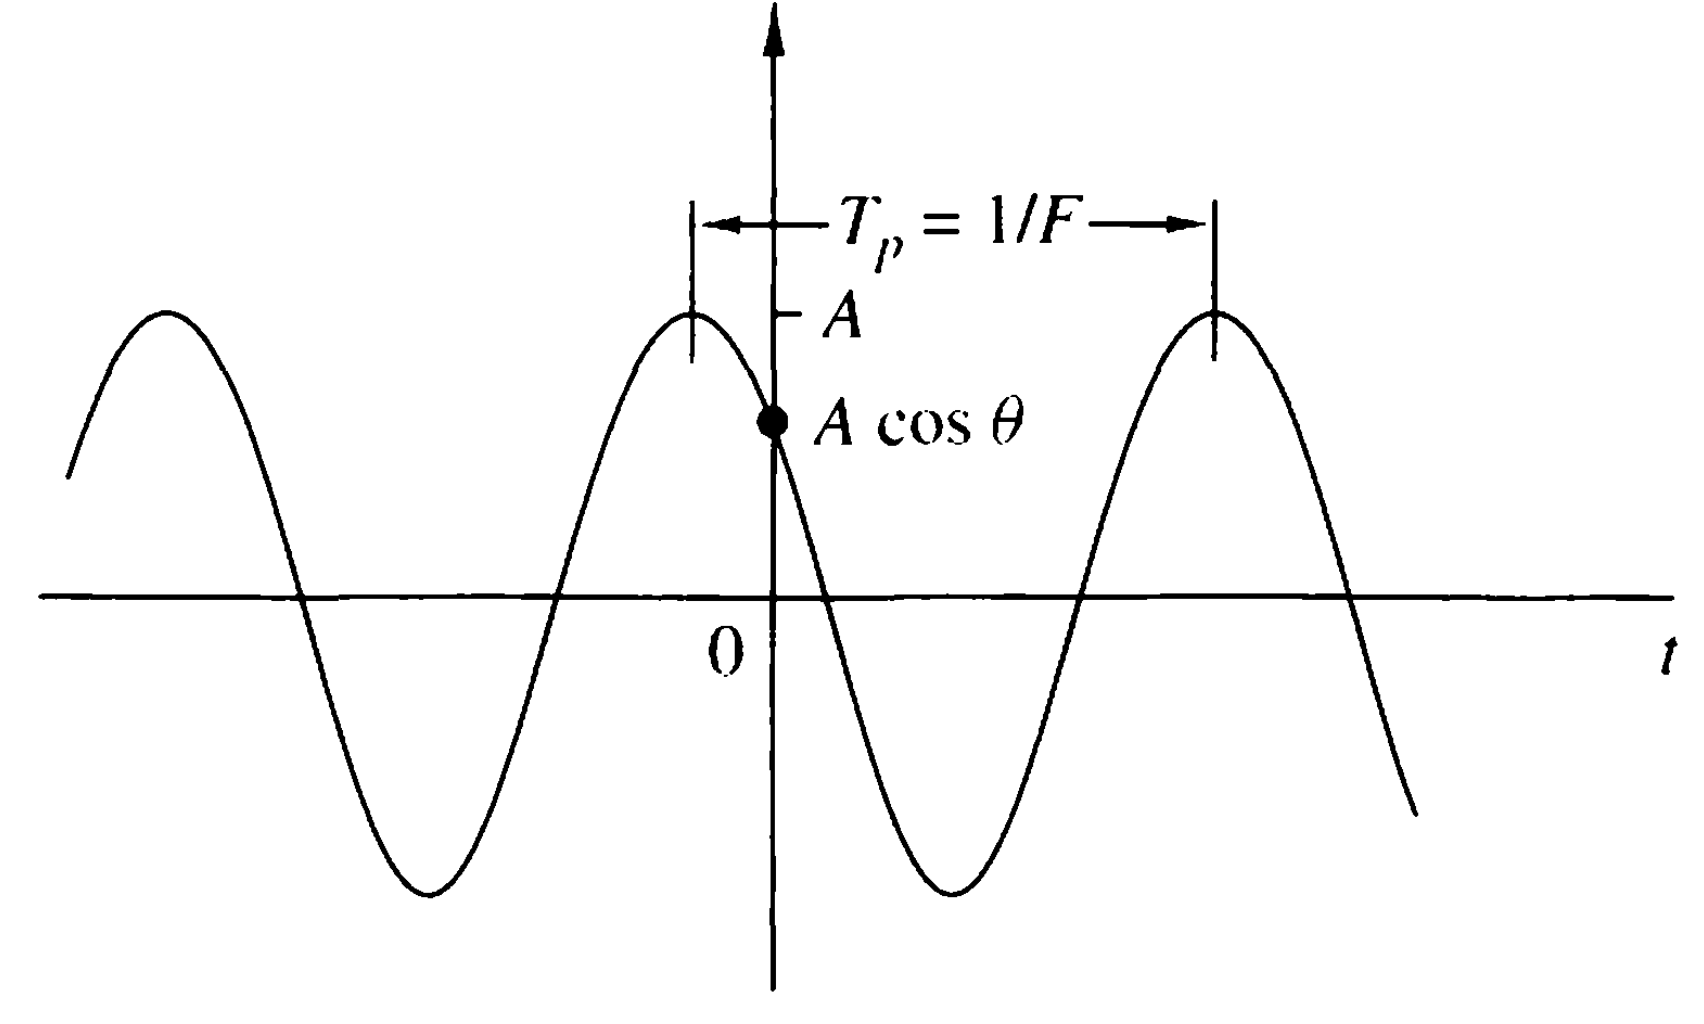
\includegraphics[width=0.48\textwidth]{img/sampling/analog_cosine.png}
        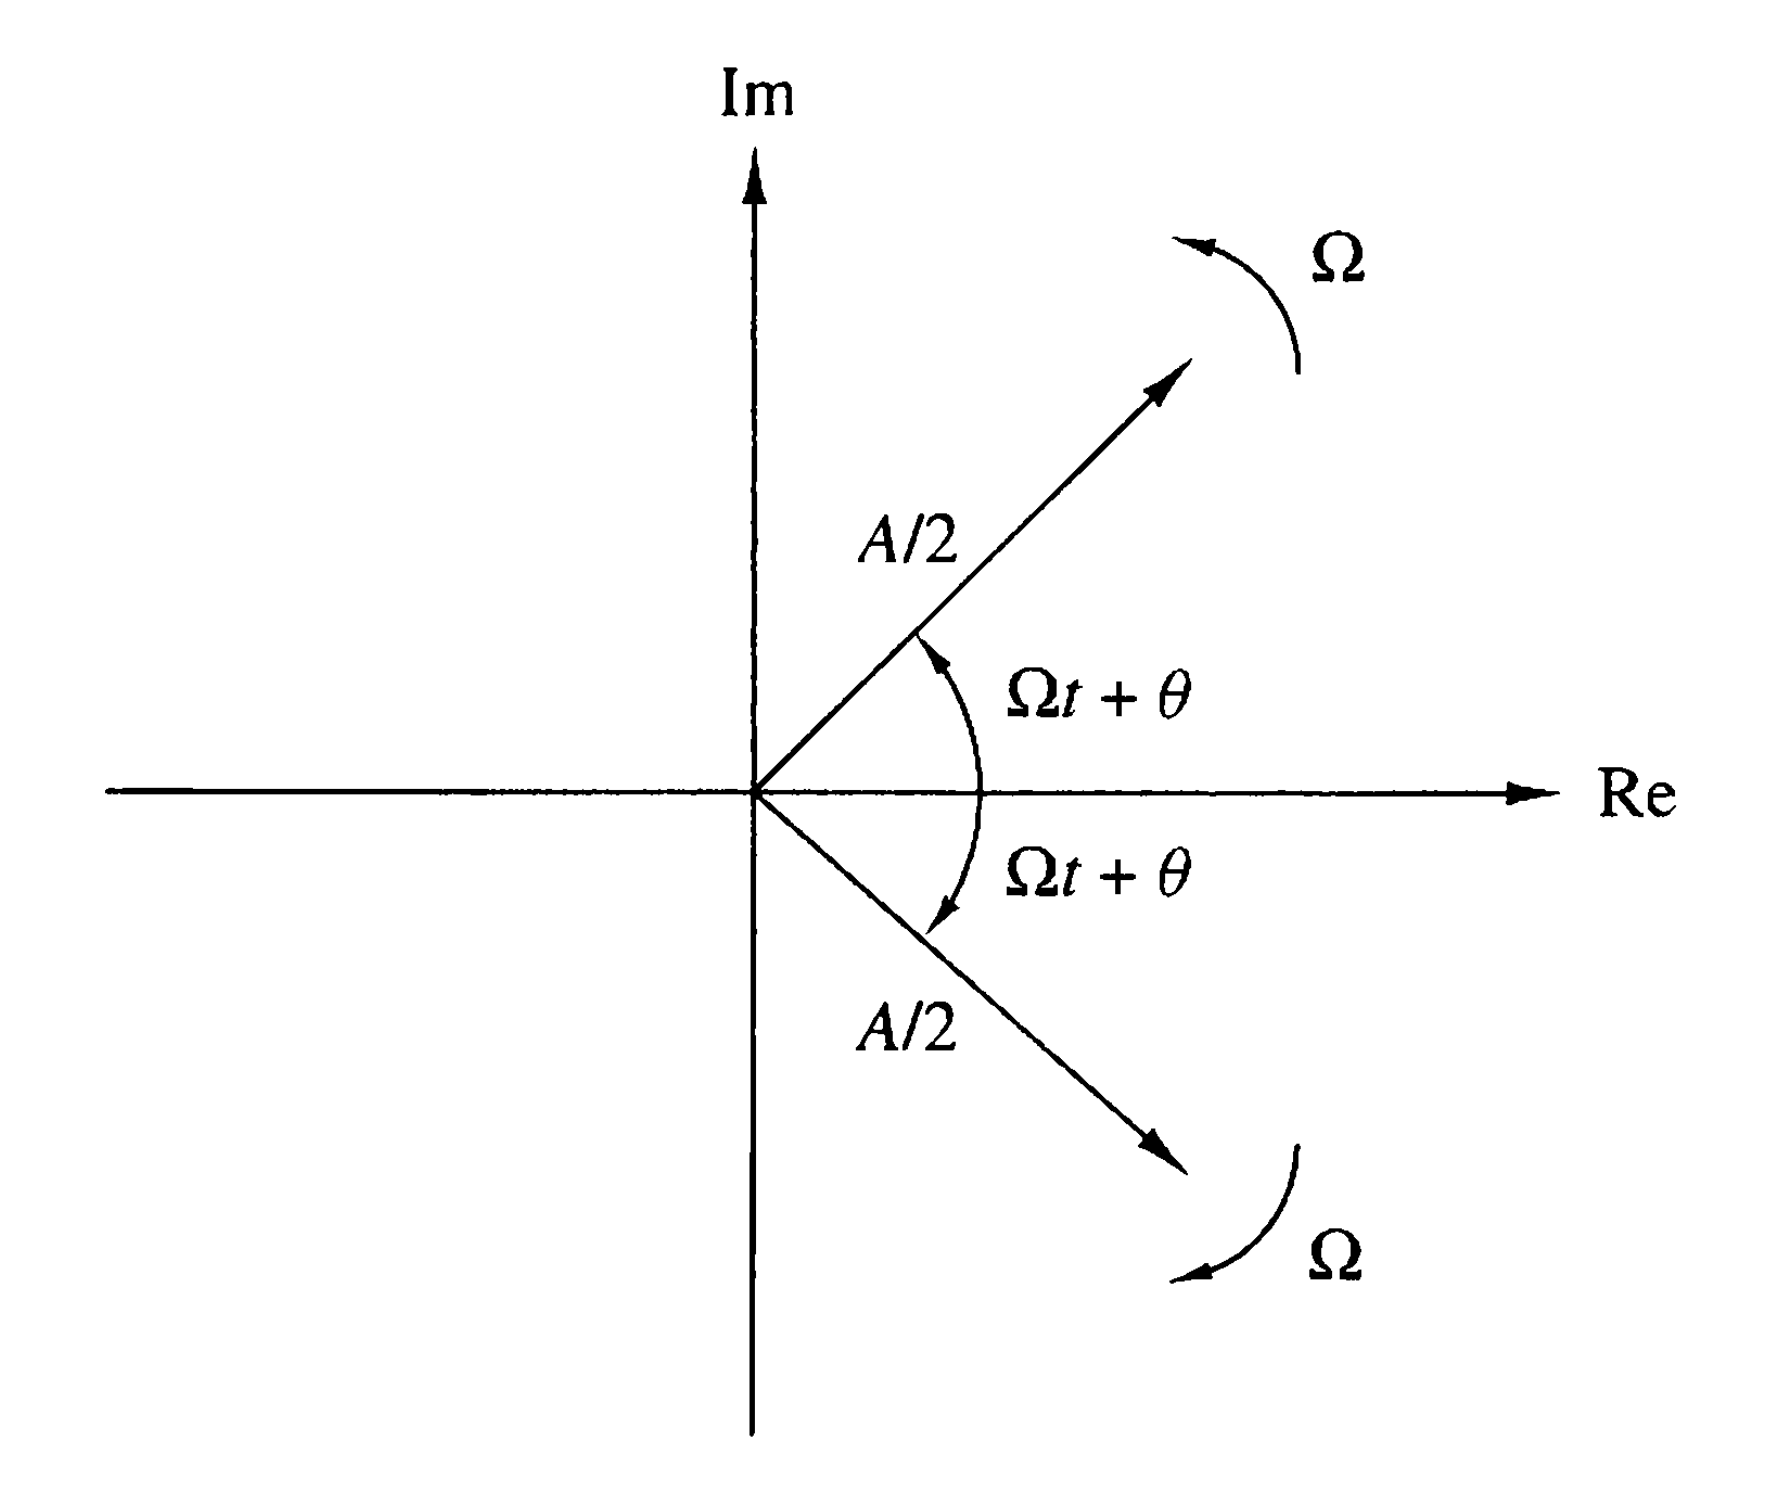
\includegraphics[width=0.48\textwidth]{img/sampling/two_phasors.png}
    \end{center}
    \caption{$x_a(t) = A \cos(2 \pi F t + \theta)$, Quelle: \cite{proakis2013}}\label{fig:analog_cosine}
\end{figure}
%
Es gibt noch eine alternative Darstellung von der obigen Funktion durch die Addition von zwei \emph{Phasoren} als
\[
    x_a(t) 
        = A \cos(2 \pi F t + \theta) 
        = \frac A2 \exp(\jmath (\Omega t + \theta)) 
            + \frac A2 \exp(- \jmath (\Omega t + \theta)).
\]
Da die beiden "uberlagerten Phasoren so interpretiert werden k"onnen als rotierten diese in gegens"atzliche Richtungen, ist es gerechtfertigt der physikalischen Intuition entgegen auch von \q{negativen} Frequenzen zu sprechen.
Wir erlauben also $F \in \R$, womit auch der Spezialfall $T_p = \infty$, also $x_a(t) = A$ abgedeckt ist.
%
\subsubsection{Zeit-Diskrete Harmonische}
%
Als n"achstes gehen wir zu dem eigentlich interessanten Fall "uber, bei welchem wir von zeitdiskreten harmonischen Signalen sprechen.
Dabei gehen wir vorerst \emph{nicht} davon aus, dass das Signal durch Abtastung eines analogen Signals entstanden ist, sondern betrachten es ganz losgel"ost f"ur sich.
In Analogie zu \eqref{eq:analog_cosine} definieren wir
%
\begin{equation}\label{eq:discrete_cosine}
    x[n] = A \cos(\omega n + \theta) = A \cos(2 \pi f n + \theta).
\end{equation}
%
Wichtig bei diskreten Signalen ist, dass ihre physikalische Interpretierbarkeit nicht direkt gegeben ist, da $n \in \Z$ nur die diskreten Werte \q{nummeriert}, also \emph{einheitenlos} ist.
Deshalb hat $f \in \R$ lediglich als Einheit \q{Zyklen pro Sample}, was man auch daran sieht, dass f"ur $f = 1$ gilt $x[n] = A \cos(2\pi n + \theta) = A \cos(\theta)$.

Es existiert nun ein wichtiger Unterschied zwischen $x[\cdot]$ von \eqref{eq:discrete_cosine} und $x_a(\cdot)$ von \eqref{eq:analog_cosine}.
Das Signal $x[\cdot]$ ist nur periodisch, falls $f$ eine rationale Zahl ist, also $f = p/q$ f"ur $p,q \in \Z$ und $q \neq 0$.

Wieso?

Ein zeitdiskrtes Signal ist periodisch, falls $x[n + N] = x[n]$ f"ur alle $n \in \Z$.
F"ur unser Signal in \eqref{eq:discrete_cosine} hei"st das also, dass
\[
    \cos(2 \pi f n + \theta) 
        = \cos(2 \pi f (n + N) + \theta)
        + \cos(2 \pi f n + 2 \pi f N + \theta)
\]
Da $\cos$ Periode $2\pi k$ f"ur $k \in \Z$ besitzt, muss $2 \pi f N = 2 \pi k$ gelten, also
\[
    f = \frac kN.
\]
